\chapter{Design and Implementation}

\section{OV7670 sensor controller}
\subsection{Overview}
To prove that the interface was suitable for image sensors a 640 x 480 OV7670 CMOS sensor was used to capture real-time image data... The Omnivision OV7670 is a small, low-cost CMOS sensor originally design for use in mobile phones which has seen popularity in the hobbyist electronics community due to its availability and ease of use. These factors, along with the wealth of documentation available contributed to its inclusion in this proof-of-concept system. As mobile phone at the time lacked the power to do image processing themselves, the OV7670 contains built-in hardware for image enhancements such as de-bayering, lens correction and noise removal, making it surprisingly complex. The OV7670 was included solely to demonstrate the effectiveness of the interface in a real camera system, thus these features are not used.

\begin{figure}
  \centering
  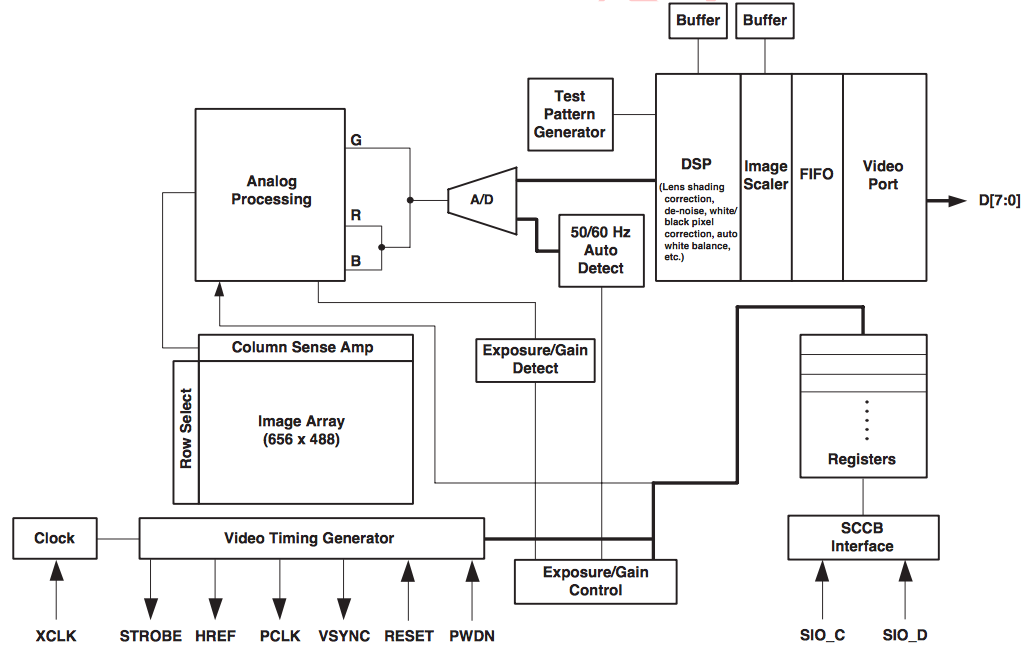
\includegraphics[width=1\textwidth]{./img/ov7670_block_diagram.png}\par
Source: Omnivision OV7670/OV7171 1.0 Specification
  \caption{Functional block diagram of Omnivision's OV7670 CMOS image sensor.}
  \label{fig:ov7670_block_diagram}
\end{figure}

Figure \ref{fig:ov7670_block_diagram} outlines the key functional blocks inside the OV7670. Light is captured by a 656 x 488 array over a specific duration of exposure. From here it is read out one row at a time into the analogue processing block which performs white-balance adjustments and amplifies the signal to increase sensitivity. From here it is digitised and fed into an image processing block for lens correction, de-noising and various other enhancements. Image scaling is also performed, before it is piped into a \gls{fifo} buffer ready for output on the 8-bit parallel video interface. The pixel size depends on the pixel format used: the RAW format only uses 8 bits and a single pixel can be output each clock cycle, while the RGB 4:2:2 and YUV 4:2:2 formats require 16 bits, thus taking two clock cycles per pixel. To construct a complete frame from the output pixels we require some additional information provided by the video timing generator in the form of vertical and horizontal synchronisation signals. The synchronisation signals in Figure \ref{fig:ov7670_timing} can be used to keep track of which the starting point of the each frame, and signals whether or not the pixel data on \texttt{D} can be sampled. 

\begin{figure}
  \centering
  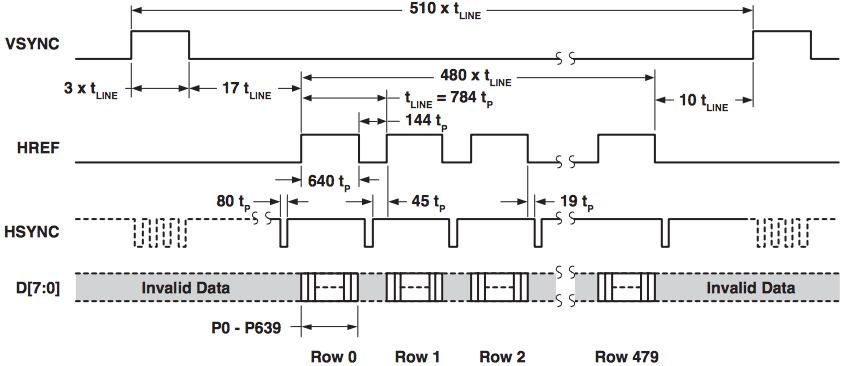
\includegraphics[width=1\textwidth]{./img/ov7670_timing.png}\par
Source: Omnivision OV7670/OV7171 1.0 Specification
  \caption{OV7670 timing diagram. The \texttt{VSYNC} signal pulses shortly before the start of each frame. \texttt{HREF} is high to indicate the data on output \texttt{D} is valid.}
  \label{fig:ov7670_timing}
\end{figure}

\subsection{\texttt{ov7670\_controller} module}
The OV7670 contains a set of internal registers to configure all aspects of its operation. In order to set the output format to 640 x 480 RAW the correct registers must be set using the \gls{sccb} protocol --- a direct clone of I\textsuperscript{2}C, renamed for licensing / IP reasons. As we are only interested in writing to specific registers there is no need to implement bidirectional I\textsuperscript{2}C communication. To drive the \gls{sccb} interface the \texttt{ov7670\_controller} module utilises I\textsuperscript{2}C code written by Mike Fields (http://hamsterworks.co.nz/mediawiki/index.php/Zedboard\_OV7670). Table \ref{table:ov7670_register_settings} lists the register settings used to configure the OV7670 for 640 x 480 RAW output at 30 \gls{fps}. On powerup, the \texttt{ov7670\_controller} module performs the following actions for each register it configures:

\begin{enumerate}
    \item Pull \texttt{SDA} low to signal master is about to send
    \item Send 8-bit address frame with value 0x42
        \begin{itemize}
            \item \texttt{Bits 7--1}: OV7670 I\textsuperscript{2}C slave address \texttt{0x21}
            \item \texttt{Bit 0}    : \texttt{R/W = 0} to write to register) 
        \end{itemize}
    \item Pause to allow OV7670 to acknowledge address frame
    \item Send 8-bit data frame with address of configuration register
    \item Pause to allow OV7670 to acknowledge data frame
    \item Send a second data frame with value to write to configuration register
    \item Pause to allow OV7670 to acknowledge data frame
\end{enumerate}

The \texttt{ov7670\_controller} module contains a 'dumb' I\textsuperscript{2}C controller --- it ignores all responses from the slave and stops as soon as it has finished configuring the OV7670 registers. For the sake of simplicity, the register configuration can be re-triggered by asserting the reset signal. Not implementing intelligence to deal with frame retransmits due to errors simplifies the design significantly, while still allowing the user to manually re-trigger register configuration if anything does go wrong. Once the configuration has been written the \texttt{ov7670\_controller} module asserts the \texttt{start\_capture} signal to notify the \texttt{ov7670\_capture} module that the OV7670 is initialised and properly configured.

\begin{table}
    \begin{tabular}{llll}
    Register            & Address   & Value     & Description                       \\
    COM7                & 0x12      & 0x80      & Reset all registers to defaults   \\
    CLKRC               & 0x11      & 0x01      & Input clock prescaler divide-by-four, disable PCLK doubling (PCLK will be \(f_internal / 2\)) \\
    DBLV                & 0x6B      & 0x7A      & Input clock PLL x4                \\
    COM7                & 0x12      & 0x01      & Output format 640 x 480 Bayer RAW \\
    COM3                & 0x0C      & 0x00      & Disable output scaling            \\
    COM14               & 0x3E      & 0x00      & No PCLK scaling                   \\
    SCALING\_XSC         & 0x70      & 0x3A      & Magical horizontal scale factor   \\
    SCAKING\_YSC         & 0x71      & 0x35      & Magical vertical scale factor     \\
    SCALING\_DCWCTR      & 0x72      & 0x11      & Downsample by 2           \\
    SCALING\_PCLK\_DIV    & 0x73      & 0xF0      & No PCLK scaling           \\
    SCALING\_PCLK\_DELAY  & 0xA2      & 0x02      & Scaling output delay 2    \\
    \end{tabular}
    \caption{(Based on values in OV7670 datasheet and implementation guide)}
    \label{table:ov7670_register_settings}
\end{table}

\subsection{\texttt{ov7670\_capture} module}
\marginpar{Code snippets required!}
Given that the purpose of a standardised image sensor interface is to provide video data in a format which can be paired with any image sensor device, it stands to reason that the data must be converted to a different format at some point. The task of the \texttt{ov7670\_capture} module is to capture pixels from the OV7670's parallel video interface and pass them on to the \texttt{i\_buf\_controller} module detailed in Section \ref{sec:framebuffer_dma} for storage in the framebuffer where they are processed by the DVI encoder. Originally the \texttt{ov7670\_capture} module had direct control over the memory, however this functionality was moved to the \texttt{i\_buf\_controller} module, reducing the \texttt{ov7670\_capture} to a passthrough or level conversion device.

To transfer frames between different blocks inside the \gls{fpga}, uses the standard VESA video interface: a pixel clock to signal when a new pixel is available, parallel data for pixels, horizontal sync for signalling end-of-line, vertical sync for signalling end-of-frame, and additionally a data valid signal which marks exactly when the active video period begins---greatly simplifying the design. Without this signal a timing recovery block would be needed to measure the frequency of \texttt{vsync} and \texttt{hsync} pulses to determine the resolution of the video and thus where the active video period begins and ends.

The OV7670's video interface is very similar, however some signals are lacking and others function differently as summarised in Table \ref{table:ov7670_video_interface}. 

\begin{table}
  \begin{tabular}{lll}
  OV7670 signal   & VESA equivalent & Description                                           \\
  d[7:0]          & d[7:0]          & Pixel data remains the same                           \\
  vsync           & vsync           & OV7670 vsync is active-high, VESA vsync is active-low \\
  href            & vde             & href is active-low, vde is active-high                \\
  N/A             & hsync           & OV7670 lacks a href signal
  \end{tabular}
  \caption{The OV7670 video interface is very similar to the VESA interface, however minor signal conversions are required.}
  \label{table:ov7670_video_interface}
\end{table}

\marginpar{Write about shutter\_sync generation}


\marginpar{NEEDS A PICTURE OF OV7670 MODULE!}

\section{Framebuffer DMA processor}
\label{sec:framebuffer_dma}

A framebuffer is a portion of memory which holds the current frame, allowing the hardware blocks either side to act in complete isolation. Both sides of the link use framebuffers, though their purpose differs. On the receiver side the framebuffer stores each frame before it is written to flash storage. Firmware inside the Zynq \gls{ps} \marginpar{Explain the Zynq PS} can draw to the frame in real-time, adding helpful indicators such as the currently connected sensor module and gridlines to aid the photographer's composition process. On the transmitter side the framebuffer serves a different purpose. A critical flaw in the design of the \gls{dvi} receiver causes the link to break if the incoming pixel clock is less than \SI{40}{\mega\hertz} --- a potential issue because the OV7670's pixel clock is only \SI{12}{\mega\hertz}. To mitigate this, the transmitter sends out duplicate frames, thus bringing the pixel clock up into the region required for correct operation.

The space required to store frames is a direct function of the image resolution. As the OV7670 outputs frames in 640 x 480 resolution, a \SI{307.2}{\kilo\byte} framebuffer is required. While \glspl{fpga} usually contain a small amount of internal block RAM, there is insufficient space for storing an entire frame. Though its access is significantly more complicated, the Zynq-7000 includes a hard DDR controller which can be utilised to store the frames in external DDR3 memory instead --- the Zybo development board contains \SI{512}{\mega\byte} of RAM, which is more than sufficient for storing a single frame.

\marginpar{Diagram of internal Zynq arch - access to DDR}

\subsection{AXI}
Due to the internal architecture of the Zynq-7000, external RAM is only accessible from the \gls{ps}, thus incoming frames which are processed by the \gls{pl} must be fed into the \gls{ps} before they can be stored in the RAM. Fortunately the \gls{pl} and \gls{ps} are able to exchange data using the \gls{axi} interface, which was designed to provide a single interconnect for IP across all domains. While there are several different variants of \gls{axi} (a comparison of which is found in Table \ref{table:axi_comparison}), they all operate in fundamentally the same way. \gls{axi} is used to connect a master device to a slave device using one or more channels which are used to carry out transactions. A standard AXI4 connection will consist of five channels:
\begin{itemize}
  \item Read Address Channel
  \item Write Address Channel
  \item Read Data Channel
  \item Write Data Channel
  \item Write Response Channel
\end{itemize}
(http://www.xilinx.com/support/documentation/ip_documentation/axi_ref_guide/latest/ug1037-vivado-axi-reference-guide.pdf)

\begin{table}[]
\centering
\caption{Comparison of AXI interfaces. Adapted from (http://www.xilinx.com/support/documentation/ip_documentation/axi_ref_guide/latest/ug1037-vivado-axi-reference-guide.pdf).}
\label{table:axi_comparison}
\begin{tabular}{llll}
              & AXI4                               & AXI4-Lite                      & AXI4-Stream                \\
Dedicated for & High-performance and memory-mapped & Register-style interfaces      & Non-address based IP       \\
Burst         & Up to 256                          & 1                              & Unlimited                  \\
Data width    & 32 - 1024 bits                     & 32 / 64 bits                   & Anything                   \\
Applications  & Embedded, memory                   & Small footprint logic, control & DSP, video, communications
\end{tabular}
\end{table}

As separate channels are used for reading and writing, device communication is fully bi-directional. In addition to the address and data signals, extra signals are provided for control and synchronisation to ensure that a device can only begin a transaction when the other device is ready. Figure \ref{fig:axi_architecture} illustrates a typical AXI4 interface. 

\begin{figure}
\centering
\begin{subfigure}{.5\textwidth}
  \centering
  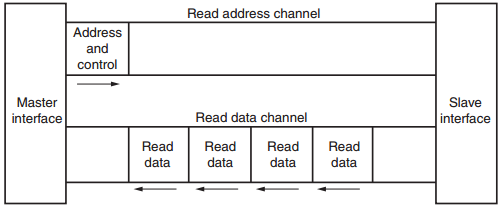
\includegraphics[width=.4\linewidth]{./img/axi_read.png}
  \caption{Read Channel}
\end{subfigure}%
\begin{subfigure}{.5\textwidth}
  \centering
  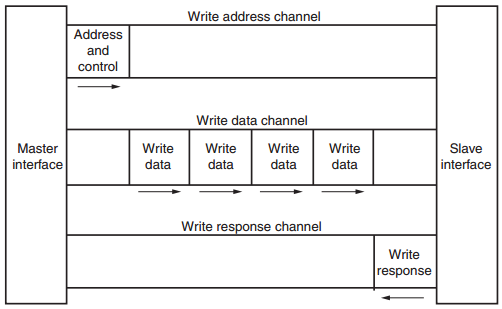
\includegraphics[width=.4\linewidth]{./img/axi_write.png}
  \caption{Write Channel}
\end{subfigure}
\caption{Architecture of AXI4 Read and Write Channels. (http://www.xilinx.com/support/documentation/ip_documentation/axi_ref_guide/latest/ug1037-vivado-axi-reference-guide.pdf)}
\label{fig:axi_architecture}
\end{figure}

All hardware inside the Zynq can be addressed from the \gls{ps} provided it has been connected via \gls{axi}. AXI requires all devices to be assigned an address which complies with the address map in Table \ref{table:zynq_address_map}. For example, the \gls{axi} master port \texttt{M\_AXI\_GP0} on the \gls{ps} has the address range \texttt{0x4000_0000} to \texttt{0x7FFF_FFFF}. Any \gls{axi} slave devices in the \gls{pl} assigned an address in this range can be accessed from the \gls{ps}. Conversely, any \gls{axi} master devices in the \gls{pl} connected to the \gls{ps} slave port \texttt{S\_AXI\_HP0} can access most of the DDR address range.

\begin{table}[]
\centering
\caption{Zynq-7000 system-level address map. (http://www.xilinx.com/support/documentation/user_guides/ug585-Zynq-7000-TRM.pdf)}
\label{table:zynq_address_map}
\begin{tabular}{lllll}
Address range                             & CPUs and ACP & AXI\_HP & Other bus masters & Notes                                                 \\
\multirow{4}{*}{0000\_0000 to 0003\_FFFF} & OCM          & OCM     & OCM               & Address not filtered by SCU and OCM is mapped low     \\
                                          & DDR          & OCM     & OCM               & Address filtered by SCU and OCM is mapped low         \\
                                          & DDR          &         &                   & Address filtered by SCU and OCM is not mapped low     \\
                                          &              &         &                   & Address not filtered by SCU and OCM is not mapped low \\
\multirow{2}{*}{0004\_0000 to 0007\_FFFF} & DDR          &         &                   & Address filtered by SCU                               \\
                                          &              &         &                   & Address not filtered by SCU                           \\
\multirow{2}{*}{0008\_0000 to 000F\_FFFF} & DDR          & DDR     & DDR               & Address filtered by SCU                               \\
                                          &              & DDR     & DDR               & Address not filtered by SCU                           \\
0010\_0000 to 3FFF\_FFFF                  & DDR          & DDR     & DDR               & Accessible to all interconnect masters                \\
4000\_0000 to 7FFF\_FFFF                  & PL           &         & PL                & General Purpose Port \#0 to the PL, M\_AXI\_GP0       \\
8000\_0000 to BFFF\_FFFF                  & PL           &         & PL                & General Purpose Port \#1 to the PL, M\_AXI\_GP1       \\
E000\_0000 to E02F\_FFFF                  & IOP          &         & IOP               & I/O Peripheral registers                              \\
E100\_0000 to E5FF\_FFFF                  & SMC          &         & SMC               & SMC Memories                                          \\
F800\_0000 to F800\_0BFF                  & SLCR         &         & SLCR              & SLCR registers                                        \\
F800\_1000 to F880\_FFFF                  & PS           &         & PS                & PS System registers                                   \\
F890\_0000 to F8F0\_2FFF                  & CPU          &         &                   & CPU Private registers                                 \\
FC00\_0000 to FDFF\_FFFF                  & Quad-SPI     &         & Quad-SPI          & Quad-SPI linear address for linear mode               \\
\multirow{2}{*}{FFFC\_0000 to FFFF\_FFFF} & OCM          & OCM     & OCM               & OCM is mapped high                                    \\
                                          &              &         &                   & OCM is not mapped high                               
\end{tabular}
\end{table}

\marginpar{Include address map of actual design}

\subsection{Linebuffers}
Due to the high complexity of the DDR controller, memory operations are not instantaneous and have non-deterministic latencies, thus an additional buffer must be placed between the incoming frames from the \texttt{ov7670\_capture} block and framebuffer, and a second between the framebuffer and the \texttt{rgb2dvi} module.

Each line of the input frame is written into a \SI{4096}{\kilo\bit} linebuffer pixel-by-pixel. 

During the blanking period an interrupt on the \gls{ps} is triggered 

\subsection{\texttt{i_buf_controller} module}

\subsection{AXI CDMA and buffer control firmware}


\marginpar{Diagram of OV7670 -> framebuffer -> DVI isolation, and DVI -> framebuffer -> SD / screen}



\section{DVI encoder}

\marginpar{Include formula for exact throughput, and pixel clocks used for OV7670}

\section{DVI decoder}
\section{EDID subsystem}
\section{Exposure sync subsystem}
\section{Flash storage manager}
\section{Viewscreen controller}
\section{Test pattern generator}
\section{Sequence detector}